\documentclass[TeamE-eindrapport]{subfiles}
\usepackage{graphicx}

\begin{document}
	\chapter{SVM in vergelijking met andere classificatietechnieken}
	
	\section{Inleiding}
	In dit hoofdstuk zal SVM vergeleken worden met andere classificatietechnieken zoals logistische regressie. Hierbij zullen we de voordelen van SVM aantonen. Dit aan de hand van enkele figuren en formules. Ook zullen er enkele nuttige toepassingen op een dataset aangebracht worden.  
	\section{Link met logistische regressie}
	Bij het toepassen van SVM is er natuurlijk ook een foutmarge. Deze wordt de hinge loss genoemd. 
	\[\frac{1}{n}\sum_{i=1}^{n}\max[0,1-y_i(\vec{w}\cdot{\vec{x_i}} - b)]\]

	Opmerkelijk bij deze loss functie van SVM is dat hij soms gelijk is aan 0. Dit voor het geval wanneer \(y_i(\vec{w}\cdot{\vec{x_i}} - b)\geq 1\). Dit zal nog verder in detail besproken worden in een volgend hoofdstuk. Deze gevallen zijn dan ook enkel voor de punten die binnen de hyperplane vallen van toepassing. Bij logistische regressie is er ook een loss functie. De grafiek hiervan is sterk gelijkend op deze van SVM. Maar bij logistische regressie zal er nooit 0 bereikt worden. Er wordt hierbij namelijk gewerkt met de formule voor de standaardfout bij regressie. 
	
	Als we deze formules beiden in een grafiek plotten zoals op figuur \ref{fig:SVMvsLogistischeRegressie}, dan zien we dat ze opmerkelijk veel lijken op elkaar behalve dan het speciale geval waarbij het punt buiten het gebied van de hyperplane valt. Hierbij kan het punt met zekerheid juist geclassificeerd worden, omdat de fout dan 0 is. Dit is een groot verschil met logistische regressie, want hierbij kan je enkel maar een kleine foutmarge bekomen voor waarden met een heel kleine decision boundary, maar je zal nooit effectief 0 kunnen bekomen. Dit is zeker ook een voordeel van SVM tijdens classificatie en zo zijn er dus situaties waarbij we omwille van deze reden kiezen voor SVM in plaats van logistische regressie. 
	
	\begin{figure}
		\centering
		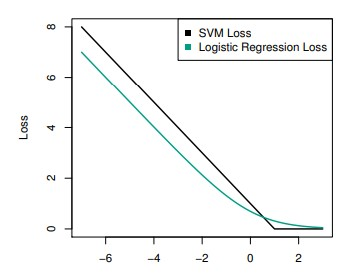
\includegraphics{SVMvsLogistischeRegressie}
		\caption{Verschil tussen de hinge loss en de standaardfout bij het toepassen van deze formules in vergelijking met de grootte van de hyperplane namelijk \(y_i(\vec{w}\cdot{\vec{x_i}} - b)\). Hierbij valt het op dat er weinig verschil is tussen beide loss functies.}
		\label{fig:SVMvsLogistischeRegressie}
	\end{figure}
	
	\section{Voordelen SVM}
	Een andere belangrijke reden om SVM te gebruiken is dat SVM zeer goed werkt bij meerdere parameters of features. Dit is iets waarbij andere classificatietechnieken veel sneller overfitten en dus in de problemen komen. Zo wordt in figuur \ref{fig:voorbeeldsvm}
	
	\begin{figure}
		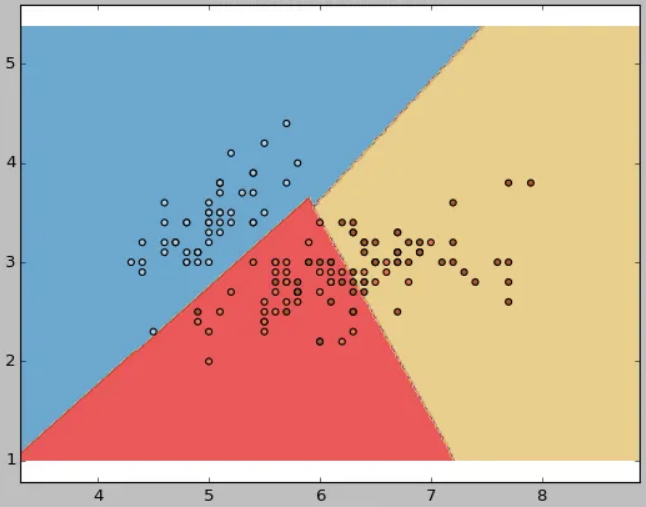
\includegraphics{VoorbeeldSVMmeerdereParameters}
		\caption{Deze figuur geeft weer hoe SVM gebruikt kan worden bij meerdere parameters.
		\label{fig:voorbeeldsvm}
			%citeer https://medium.com/@balajicena1995/support-vector-machine-with-numerical-example-8dfe81eae4f0}
	\end{figure}
	
	
\end{document}